%% ----------------------------------------------------------------
%% Design.tex
%% ---------------------------------------------------------------- 

\chapter{System Design} \label{Chapter:System Design}

System design is a fundamental process of the software development that defines the architecture, the components and the interface of a system to satisfy specific user requirements. This chapter will firstly describe the sources of open datasets and how they will be utilized in this system. Then it will detailedly discuss the system design based on the background research and the system. Finally, the user interface design of this system will be introduced using some typical wireframes drawings.

\section{Open Datasets}
After identifying the functional requirements, it is necessary to search for or collect relevant open datasets and use them in data visualisation. Due to time constraints, public APIs (Application program interfaces) become the first choices of this system. The advantage of APIs is that the developers do not need to pre-process data and design database, which can save much time in the software development lifecycle. Also, the real-time access to APIs can ensure that the latest data can be obtained. However, it may be a problem that some open APIs are likely to restrict unlimited access or require users to pay for more operations.

\subsection{Unistats API}

Unistats API is an open API provided by Higher Education Statistics Agency (HESA). This API provides comparable sets of information about university courses in the UK, such as course mode, tuition fees and living expenses. Moreover, it provides the details of the location of universities or courses, including the latitude and longitude. Therefore, this API was used to provide international students with information on universities and courses.


\subsection{Google Maps API
}

Google Maps provides some map APIs that allow the developers to add different functions to the embedded Google Map on the web pages. In this system, Google Maps Distance Matrix API was used to estimate travel time and distance between universities and several metropolises, like London and Edinburgh. Besides, Google Map Places API was used to provide information about infrastructure around universities.


\subsection{OpenWeatherMap API
}

Although the historical weather data would offer a better understanding of weather in cities, it is hard to find available open datasets or free open APIs about the historical weather of cities in the UK. Most open datasets, like Met Office, only provide historical weather data of observation stations instead of that of cities. As a result, the information about weather provided in this system was the weather forecast for next hours and next 14 days, and the data came from OpenWeatherMap API.

\subsection{Police API
}

Police.uk provides a Police API that gives the public free access to open data about crime and policing in England, Wales and Northern Ireland. Specifically, the Police API allows the public to retrieve data about crime or policing within different locations or categories. Hence, the police API was used in this system to provide international students with detailed information on criminality or safety of cities. 

\subsection{THE University Ranking Table 
}

Due to the lack of related open APIs, the dataset about university ranking was from THE university ranking tables, which included some ranking criteria, such as teaching quality and student experience.  The dataset was originally manipulated using Open Refine. After data manipulation, it was saved as a CSV file and displayed in a table.

\section{Architecture Design
}


The architecture design is a process that describes the structure, behaviour and more views of a system and it has a great impact on the performance, robustness, distributability, and maintainability of a system \cite{5_sommerville_2011}. AngularJS, a kind of front-end JavaScript framework, is used to implement this system. More in detail, the overall architecture of this system is the model-view-viewmodel (MVVM) pattern. MVVM pattern helps separate business logic (model) from the UI (view) using the view model, so it allows the developers to write better organized, and therefore more maintainable system. As Figure 5.1 shows, the MVVM pattern has three logical components (model, view and view model), which are interrelated and interact with each other. The detailed interaction between these three components will be explained in the following section.
\begin{figure}[H]
  \centering
  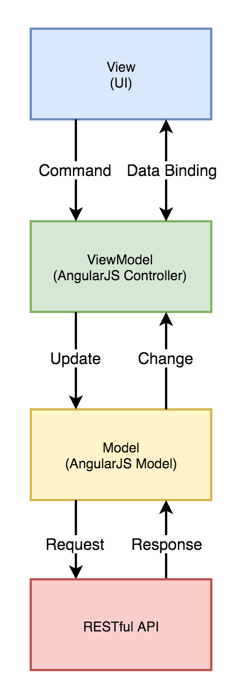
\includegraphics[width=4cm]{./img/Picture7}
  \caption{System Architecture}
  \label{Figure:figex}
\end{figure}



\section{Detailed Design}
\subsection{Use Case Diagram}
Figure 5.2 is a use case diagram shows the overview of the functional requirements provided in this system and the interactions between the users and the system. The users of this system are international students who want to get information about universities and cities for their higher education destination choices. It is noticeable that these use cases have include or extend relationships with each other. Particularly, “View University\&Course Part” and other five use cases are included in “Search universities and courses”, which means that all these six use cases can only be accomplished after searching universities and courses.

\begin{figure}[H]
  \centering
  \includegraphics[width=15cm]{./img/Picture8}
  \caption{Use Case Diagram}
  \label{Figure:figex}
\end{figure}

\subsection{Activity Diagram}
An activity diagram is a simple and intuitive representation of what happens in a workflow, what activities can be done in parallel, and whether there are alternative paths through the workflow \cite{IBM}. Therefore, an activity diagram can help understand the workflow of activities while using this system. As shown in Figure 5.3, it is clear that the workflow of this system is simple and straightforward, which makes it easy for the users to understand and use this system. Apart from the activities in the following figure, the users also can select different months and different kinds of infrastructure in criminality and infrastructure part respectively. 
 


\begin{figure}[H]
  \centering
  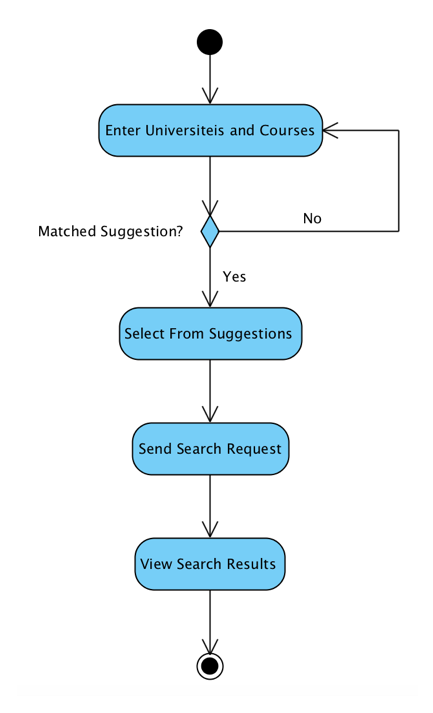
\includegraphics[width=6cm]{./img/Picture9}
  \caption{Activity Diagram
}
  \label{Figure:figex}
\end{figure}



\subsection{Sequence Diagram}
The purpose of a sequence diagram is to show interactions and communications between the objects of a system in time sequence \cite{IBM2}. Figure 5.4 presents a sequence diagram that is used to present how the components of MVVM pattern interact with each other when the users interact with the view.

\textbf{Model}: The Model, which refers to the controllers in AngularJS, is responsible for sending requests to various RESTful APIs and return related data to the view model.

\textbf{View}: The View, which refers to the user interface, is responsible for receiving commands from users and displaying the data that is supplied by the view model as result. 

\textbf{View Model}: The View Model is responsible for presenting data from the model, receiving data change of view and change the model.



\begin{figure}[H]
  \centering
  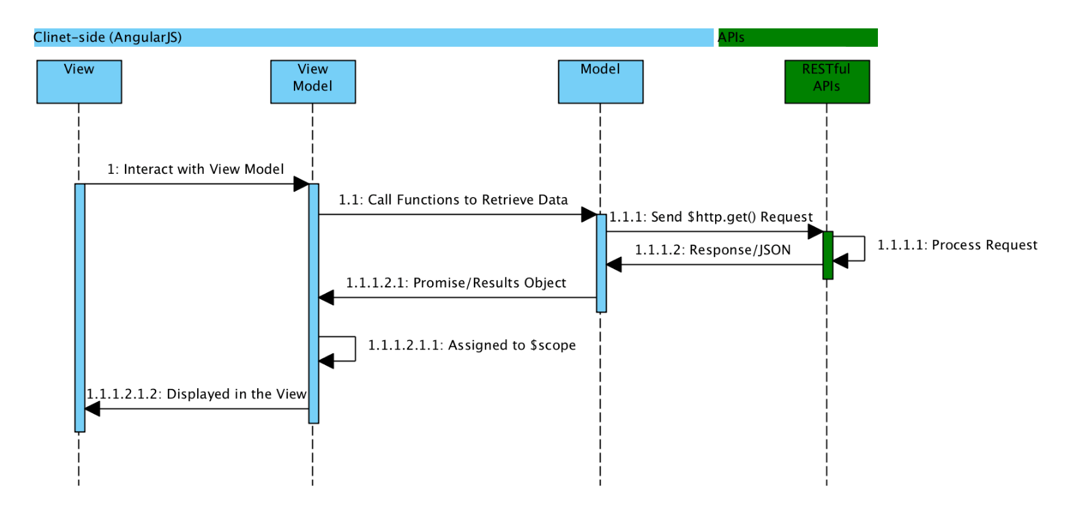
\includegraphics[width=16cm]{./img/Picture10}
  \caption{Sequence Diagram of MVVM Pattern}
  \label{Figure:figex}
\end{figure}



Moreover, Figure 5.5 is an another sequence diagram that provides information about the interactions between the browser and several open APIs used in this system. When the users send search requests via the browser, Unistats API will return data about the selected universities and courses, and the responses will be displayed on the webpage. Meanwhile, the browser will send several requests containing the geolocation data about cities, which are from Unistats API, to other open APIs. Afterwards, these APIs will return related data about cities to the browser accordingly.



\begin{figure}[H]
  \centering
  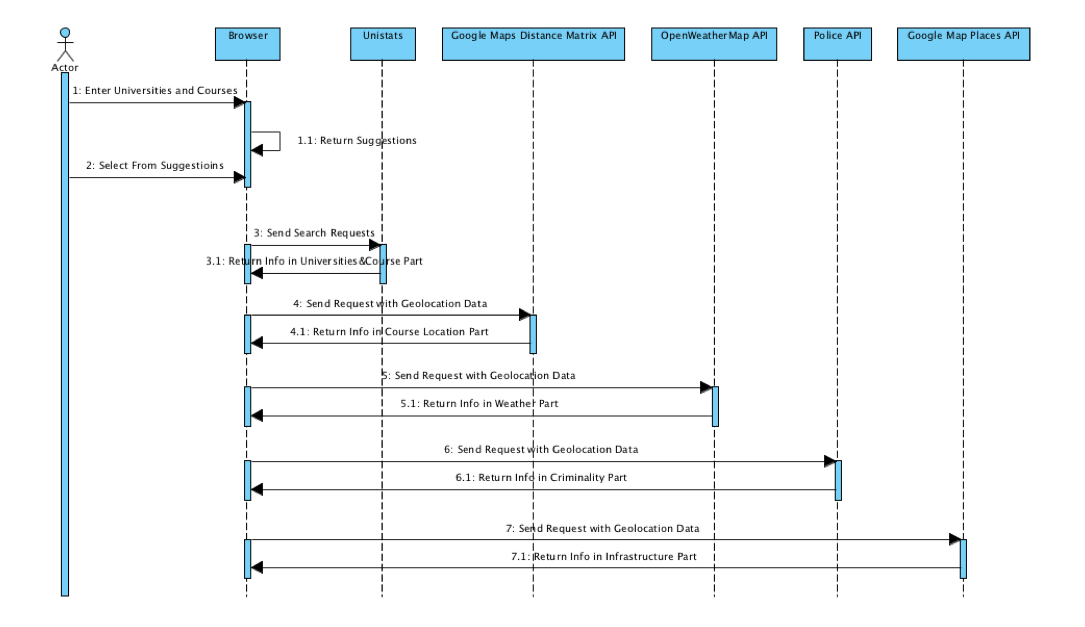
\includegraphics[width=15cm]{./img/Picture11}
  \caption{Sequence Diagram of Interaction Between Brower and Open APIs}
  \label{Figure:figex}
\end{figure}


\section{User Interface Design
}

A fundamental reality of software development is that the user interface is the system to the users \cite{ambler2000user}. Hence, the user interface is as important as the functionality that a system provides to the users. A good user interface design can make the system easy to use and understand. In this section, some typical wireframes drawings will be used to introduce the user interface design of this system.


\subsection{Layout}

The layout of the system was the first element that should be considered in the use interface design. A well-designed layout allows users to gain insights into the functionalities of the system rapidly and intuitively. There were two sections in this system, namely university section and about section. The webpage of each section can be divided into three parts as shown in Figure 5.6. The top (1) and bottom (3) of the webpage was a navigation bar and a footer, which can offer the users quick access to the sections in this system and some additional information respectively. The middle (2) of the webpage was used to display main content of each section.


\begin{figure}[H]
  \centering
  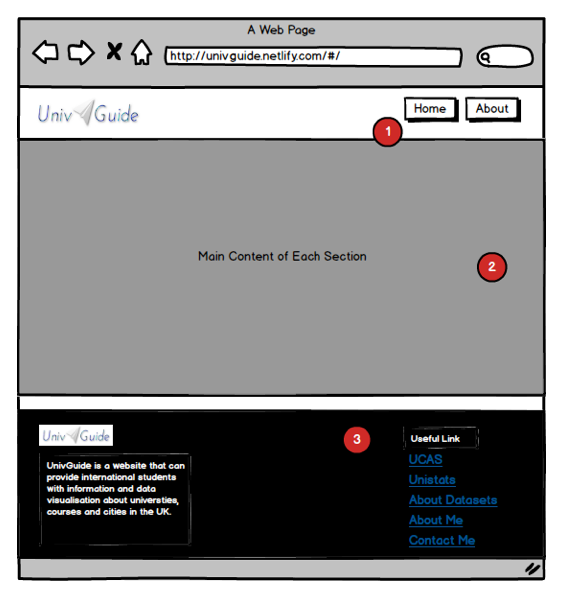
\includegraphics[width=10cm]{./img/Picture12}
  \caption{Layout}
  \label{Figure:figex}
\end{figure}



\subsection{Initial Page}
The initial page (see Figure 5.7) was designed for the users who enter this system at the first time.  It presented the overview or guide (5) of this system. Besides, the search bar (4) was placed in a prominent position because it was the most important component of this system.


\begin{figure}[H]
  \centering
  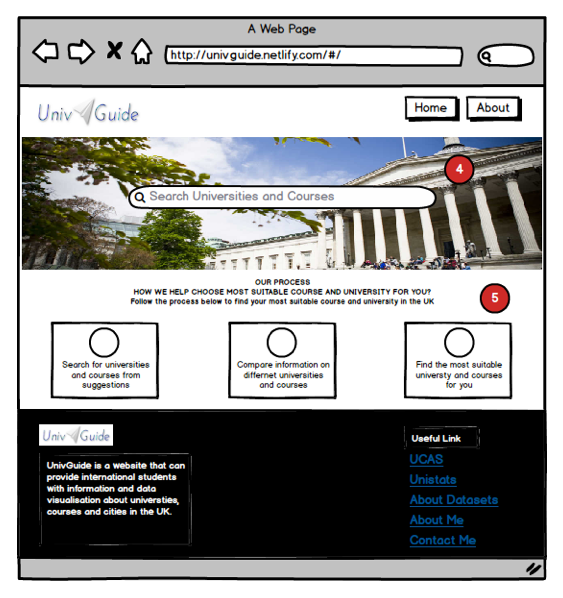
\includegraphics[width=10cm]{./img/Picture13}
  \caption{Initial Page}
  \label{Figure:figex}
\end{figure}


\subsection{University section
}

When the users search for universities or courses and select one from suggestions, the university section will replace the overview (5) of this system. The university section (see Figure 5.8) consists of search parts, namely University\&Course (6), Ranking Table (7), Course Location (8) and City Information (9). These parts are the core functionalities of this system. Specifically, University\&Course part contains information about selected universities or courses; The ranking table displays THE University Ranking; The course location part presents the location and the geographic proximity of selected universities or courses. The city information part includes information about weather, criminality and infrastructure of the cities that selected universities or courses are located in.



\begin{figure}[H]
  \centering
  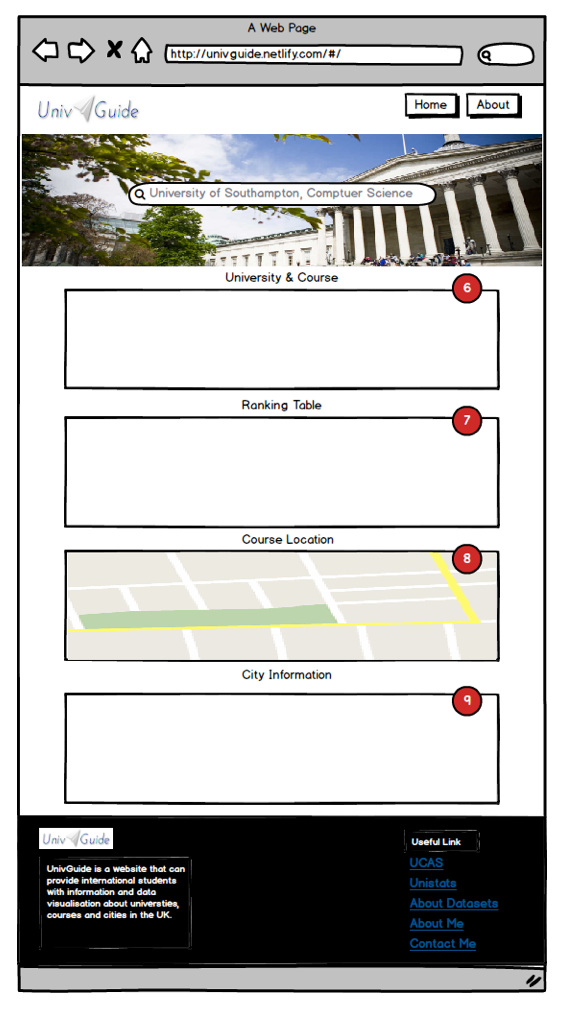
\includegraphics[width=10cm]{./img/Picture14}
  \caption{University Section}
  \label{Figure:figex}
\end{figure}



\subsection{About section
}

The about section (see Figure 5.9) provided some additional information about this system, such as the goal of this system (10), the data sources (11) and the people involved in its development (12).


\begin{figure}[H]
  \centering
  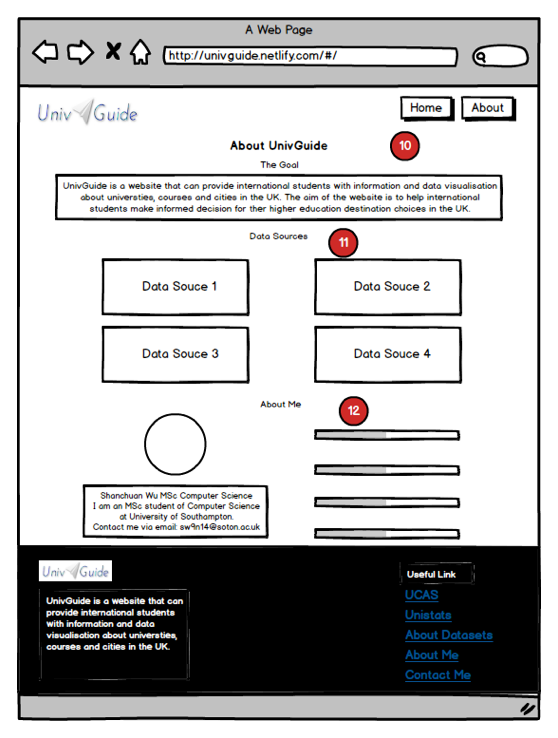
\includegraphics[width=10cm]{./img/Picture15}
  \caption{About Section}
  \label{Figure:figex}
\end{figure}



\section{Summary}

This chapter firstly provides information about the sources of open datasets and explains how they are used in this system to provide information about universities and cities in the UK. Afterwards, the detailed design of this system is introduced with some UML diagrams. At last, several wireframes drawings are presented to illustrate the prototype of user interface design. 





